\chapter{Integer Linear Programming}
\section{Introduction}

The setting is very similar to the linear programs we already know. We just restrict the problems and the possible solutions a bit. As the name suggests we want integer solutions to our programs. In general it is hard to tell whether some constraint system naturally describes a polyhedron where all optimal solutions are integral, so we need to actively restrict the solution space. 

\begin{Def}[Integer Linear Program] Given\footnote{In my opinion $\R$ would be okay too} $A\in \Z^{m\times n}$, $b\in \Z^m$, $c\in \Z^{1\times n}$ find a $x\in \Z^n$ such that $Ax\leq b$ and $cx$ is maximal (or minimal)

\begin{align*}
\max \quad & cx \\
s.t. \quad & Ax \leq b\\
&x\in \Z^n
\end{align*}
\end{Def}

If we just restrict some variables to be integral and allow arbitrary values for the others we have a mixed integer linear program.

Integer linear programs allow us to model some new interesting problems that we couldn't before. The most prominent examples are 

\begin{itemize}
\item binary choices, e.g. many NP-complete problems like Knapsack require some choice. 
\item relations between variables, e.g. choose at most ten of these things $\sum x_i \leq 10, x_i\in \{0,1\}$
\item disjunctive constraints, e.g. $x\geq a$ or $y\geq b$, can be modeled by introducing a decision variable $\delta \in \{0,1\}$ and saying $x\geq a\delta$ and $y \geq b(1-\delta)$. 
\item conditional constraints, e.g. if $x>a$ then $y>b$, can be modeled using disjunctive constraints: $x\leq a$ or $y>b$
\item piecewise linear cost functions become possible by introducing decision variables that decide on the piece we're in.
\end{itemize}

Integer Linear Programs are harder to solve than normal linear programs. Rounding, for example, doesn't work very well, as the cost difference between the optimal integral solution and an optimal fractional solution can be quite large.

\begin{thm} Finding a feasible solution for an ILP is NP-complete.
\end{thm}

\begin{pr} We prove by a reduction from SAT that ILP is NP-hard. For a given formula in CNF we construct an ILP like this:

For each variable $v_j$ in the formula we introduce $z_j \in \{0,1\}$ in our ILP, with the natural interpretation of the value of $z_j$. For every clause $C_i$ let $J^+_i$ be the number of positive and $J^-_i$ be the number of negated variables in clause $C_i$.

The ILP for the formula is then

\begin{align*}
\max \quad & 42 \\
s.t. &\sum_{j\in J^+_i} z_j + \sum_{j\in J^-_i} (1-z_j) \geq 1 && \forall i\\
&z_j \in \{0,1\}
\end{align*}

The constraints make sure that in every clause at least one positive variable is 1 or one negative variable is 0. If the feasible region of the LP is nonempty then the formula is satisfiable. The formal proof is omitted as it is rather obvious.

To show NP completeness we need to show that ILP is in NP. In the 0-1 case it is rather obvious that we can use any feasible solution as a polynomial witness. In the general case we would need to show that the entries in the solution vector are polynomially bounded. This is quite complicated but follows from the polynomial running time of the ellipsoid method. We will omit that proof here.
\qed \end{pr}

NP-completeness is a worst-case statement. Some ILPs can be solved efficiently. We'll talk about conditions for that.

\section{Integer hull of a polyhedron}

The integer hull of a polyhedron is the set of feasible solutions $\{x | Ax\leq b, x\in \Z^n\}$. As we know $\{x|Ax\leq b\}$ is a polyhedron. Let $P_I = \{x| Ax\leq b\}_I$ be the convex hull of the integral vectors in $P$. See figure \ref{Fig:integerHull}

\begin{figure}[hbt]
\begin{center}
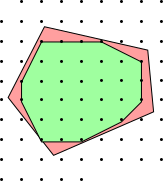
\includegraphics{./images/integerHull}
\end{center}
\caption{The integer hull of a polyhedron}
\label{Fig:integerHull}
\end{figure}

We make the following propositions:

\begin{enumerate}
\item If $P$ is bounded then so is $P_I$
\item If $A$ contains only rational numbers, $P$ is rational. For rational $P$ the integer hull is also a polyhedron.
\item If $P$ is unbounded and $A,b$ arbitrary real then $P_I$ is not necessarily a polyhedron.

For example the polyhedron

\[P=\{(x,y)|y\leq \sqrt{2} x\}\]

Does not have an integer hull. The integral points that are closest to the line defined by $y=\sqrt 2 x$ are $\{(x,\lfloor \sqrt 2 x\rfloor)|x\in \Z\}$, in particular $(0,0)$ is exactly on the line. Their ratio approximates $\sqrt 2$ from below. So for increasing $x$, $(x,\lfloor \sqrt 2 x \rfloor)$ defines a line with $(0,0)$ that has a steeper slope than all lines $(0,0)$ to $(x',\lfloor \sqrt 2 x' \rfloor), x'<x$. So only $(0,0)$ and $(x,\lfloor \sqrt 2 x \rfloor)$, for $x\rightarrow \infty$, are on the convex hull.

That means it is not possible to find a line with rational slope that defines the convex hull, as for every slope $p/q$ there is some $x$ such that $\sqrt 2 - (\lfloor \sqrt 2 x \rfloor/x) < \sqrt 2 - p/q$. Hence the integer hull is not a polyhedron.
\end{enumerate}

Obviously if $P=P_I$ then the solution for an ILP with feasible region $P_I$ is the same as the solution for the relaxed problem with feasible region $P$. This is the nice case where we can solve the ILP optimally in polynomial time using the methods we already know.

\begin{Def} A polyhedron $P$ is called integral if $P=P_I$\end{Def}

\begin{thm}\label{Thm:polyIntegrality} A rational polytope $P$ is integral iff for any integral cost vector $c$ the optimal point $x$ is also integral.

\[\exists x\in P,x\in \Z^{n\times 1}\forall c\in \Z^{1\times n}, y \in P:\ cx\geq cy\] 
\end{thm}

If the cost vector $c$ is integral and the optimal solution $x$ is also integral, obviously $cx\in \Z$.

\begin{pr} $\Rightarrow$ If the polytope is integral all vertices are integral. Since optimal values are always attained at vertices, the optimal solution will also be integral, so that direction is easy.

$\Leftarrow$ For the other direction suppose $\max \{cx | x\in P\}\in \Z\quad \forall c\in \Z^{1\times n}$. We want to show that all vertices in the polytope are integral.

Choose $c$ s.t. it has a unique optimal solution $y$. We have 

\[cy>cx + x_1 -y_1 \quad \forall x\in P,x\neq y\]

By multiplying $c$ be an arbitrary integer we can make the gap between the unique optimal solution $y$ and any other solution $x$ as large as we want, in particular large enough to make that inequality true.

We can change the cost function a bit without making $y$ nonoptimal. Let $\bar c = (c_1+1,c_{2,\ldots,n})$. We claim:

\[\bar c y > \bar c x\qquad \forall x\neq y\]

We want to compute by how much the cost changed. Since we increased the first component of $c$ we get

\[\bar c y = cy+y_1\]

Since we assumed that $cy$ is integral and our modification didn't impact integrality that equality forces $y_1$ to be integral too. We can do that for all components so they must all be integral. Since this must hold for all cost vectors it holds for all vertices and our polyhedron must be integral.
\qed \end{pr}

It is possible to extend this result to arbitrary polytopes, even those that don't have vertices.


\section{Total dual integrality}

As we said the case that $P=P_I$ is the nice case we can easily solve. In general it is hard to tell whether this is true, but for some constraint matrices we can prove that they always define integral polyhedra.

Strong duality as for linear programs does not hold for ILPs. But we have something similar for a special class of constraint matrices.

\begin{Def} A system $Ax\leq b$ is called totally dual integral (TDI) iff for each integral $c$ with bounded maximum we have

\[\max \{cx |Ax\leq b\} = \min \{\trans y b | \trans y A = \trans c, y\geq 0, y\in \Z^m\}\]

Note that $x$ doesn't have to be integral here.

The same works for $Ax\leq b, x\geq 0$ and $Ax=b, x\geq 0$
\end{Def}

Although $x$ doesn't have to be integral in the optimal solution of a TDI system, we have the following nice result:

\begin{thm} If $Ax\leq b$ is TDI and $b$ is integral, then $P=\{x|Ax\leq b\}$ is integral.
\end{thm}

\begin{pr} The proof is by contradiction. Assume $P$ is not integral and take a fractional vertex $x$ of $P$. Construct an integral cost vector $c$ such that $x$ is optimal, by taking a rational one and scaling.

In particular that means if $b\in \Z$ then the whole polyhedron is integral.
\qed \end{pr}

So if we can show dual integrality, we immediately get the integrality of the original polyhedron for all integral RHS $b$.

It is important to note that TDI is not a property of the polyhedron but instead of the system that defines it. Very much like with degeneracy we may find another system that describes the same polyhedron but is in fact TDI. 

Suprisingly there is the following theorem:

\begin{thm}\label{existsTDIsystem} For each rational polyhedron $P$, there exists a TDI system $Ax\leq b$ with an integral matrix $A$. Iff $P$ is integral then $b$ can be chosen to be integral too.
\end{thm}

Since finding feasible solutions for ILPs is NP-complete and the proof didn't make use of a nonrational constraint matrix it must be hard to find a polynomial size TDI system for the polyhedron (or no such system exists). At least that's what I suspect.

\begin{pr}[Theorem \ref{existsTDIsystem}] (From the book by Cook etc) Let $P=\{x | Mx\leq d\}$ and $M$ is integral. If $P$ is rational we can always scale the matrix up until it is integral. Now we take all conic combinations of the rows of $M$ that are integral

\[L=\{l\in \Z^n | l = \trans y M, 0\leq y\leq 1\}\]

$L$ is a finite set because we only consider only the integer points in a bounded set. Note though that $L$ is quite large in general.

We now use the elements of $L$ to construct a TDI system. For $l\in L$ let $t(l) = \max\{\trans l x | x\in P\}$, i.e. $t(l)$ is the optimal value for any point in $P$ with respect to some special, integral cost vector $l$. $t(l)$ can be found by solving one LP per $l\in L$. Note that $t(l)$ is integer if $P$ is integral.

Now comes the trick. Define the new system $Ax\leq b$ using the inequalities $\trans lx\leq t(l)$. This must be equal to $P$ because each $l$ is just a linear combination of old constraints and we defined $t(l)$ using points in $P$.

We need to show that this system is TDI, i.e. for every integral cost vector $c$ the dual has an integral optimal solution. Let $c$ be integral and chosen s.t. $z^*:=\max \{cx|x\in P\}$ is bounded. We want to construct an integral solution to $z^*=\min \{\trans yb | \trans y A = \trans c, y\geq 0\}$.

Let $y^*$ be the possibly fractional optimal dual solution for the original matrix $M$. 

\[y^* = \argmin y \{\trans y d| \trans y M = \trans c\}\]

Construct a new dual RHS vector $\bar c = \trans{(y^*-\lfloor y^*\rfloor)}M$. $\bar c$ is a convex combination of the rows of $M$. But it must also be integral since $\trans{(y^*-\lfloor y^*\rfloor)}M=\trans{y^*}M-\lfloor\trans{y^*}\rfloor M$ and we know $\trans{y^*}M=\trans c$ and the second part must be integral because we take an integral combination of an integral matrix.

However $y^*-\lfloor y^*\rfloor$ is an optimal solution for $\min \{\trans y d| \trans yM=\trans{\bar c},y\geq 0\}$. TO BE CONTINUED
\qed \end{pr}

This together with theorem \ref{Thm:polyIntegrality} has the following corollary: Let $A\in \Q^{n\times m}$, $b\in \Z^n$ and $Ax\leq b$ is TDI then $\{x|Ax\leq b\}$ is integral.

There seems to be a polynomial method to check whether a system is TDI, but I don't know how it works. See the book by Cook.

What we can do however is to have a hard look at the dual and "recognise" that it always has integral optimal solutions.

\begin{Ex} Given a directed graph $G=(V,E)$, two vertices $s,t\in V$ and the set of paths $P$ between $s,t$. We're also given a cost function $c$ on the edges. The task is to assign positive weights $y_e$ to the edges s.t. each path has accumulated cost at least 1. While doing so we want to minimize

\[\sum_{e\in E} c(e), y_e\]

One maybe recognize this as a Min-Cut problem. Formulated as a LP that is 

\begin{align*}
\min \quad & \sum_{e\in E} c(e) y_e\\
s.t. & \sum_{e\in p} y_e \geq 1 && \forall p\in P\\
&y_e \geq 0
\end{align*}

We want to show that the polyhedron $Q$ that is defined by the above constraints is integral by showing that it is TDI. To do that we construct the dual:

\begin{align*}
\max \quad & \sum_{p\in P} x_p\\
s.t. & \sum_{p,e\in P} x_p \leq c(e) && \forall e\in E\\
 & x_p \geq 0 && p\in P
\end{align*}

By looking hard at the dual we see that it defines a maximum flow problem. As we know maximum flow problems with integer capacities have integral optimal solutions. Hence we have a TDI system and the primal polyhedron must be integral, since the RHS is integral.
\end{Ex}